\documentclass[11pt]{article}

\usepackage{CMPSC465}
\usepackage{enumitem}
\usepackage{algpseudocode}
\usepackage{tikz}
\usepackage{amsmath}
\usepackage{tikz} 
\usepackage{graphicx}
\usepackage[colorlinks=true, allcolors=blue]{hyperref}
\usepackage{tkz-graph}
\PassOptionsToPackage{usenames,dvipsnames,svgnames}{xcolor}  
\usepackage{tikz}
\usetikzlibrary{arrows,positioning,automata}
\def\title{Solution 06}

\def\defeq{\mathrel{\mathop:}=}
%\usepackage{algpseudocode}
%\usepackage{algorithm}
%\usepackage[ruled]{algorithm2e}
%\usepackage{amsthm}


\def\defeq{\mathrel{\mathop:}=}
%\usepackage{algpseudocode}
%\usepackage{algorithm}
\usepackage[ruled,noline]{algorithm2e}
%\usepackage{amsthm}
\newcommand\nonl{%
  \renewcommand{\nl}{\let\nl\oldnl}}% Remove line number for one line
  
\newcommand{\aaa}[1]{\hspace{0.65cm}\parbox[t]{15.3cm}{#1}}
\newcommand{\aab}[1]{\hspace{1.15cm}\parbox[t]{15.0cm}{#1}}
\newcommand{\aac}[1]{\hspace{1.65cm}\parbox[t]{15.0cm}{#1}}
\newcommand{\aad}[1]{\hspace{2.15cm}\parbox[t]{15.0cm}{#1}}
\newcommand{\aaA}[2]{\hspace{0.5cm} {\tikz[overlay] \draw (0.1, -0.1) -- (0.1, #1 * -1.5em + 0.6em);} \parbox[t]{15.0cm}{#2}}
\newcommand{\aaB}[2]{\hspace{1.0cm} {\tikz[overlay] \draw (0.1, -0.1) -- (0.1, #1 * -1.5em + 0.6em);} \parbox[t]{15.0cm}{#2}}
\newcommand{\aaC}[2]{\hspace{1.5cm} {\tikz[overlay] \draw (0.1, -0.1) -- (0.1, #1 * -1.5em + 0.6em);} \parbox[t]{15.0cm}{#2}}
\newcommand{\aaD}[2]{\hspace{2.0cm} {\tikz[overlay] \draw (0.1, -0.1) -- (0.1, #1 * -1.5em + 0.6em);} \parbox[t]{15.0cm}{#2}}
\newcommand{\xxx}{\par\vspace{0.1cm}}
\usepackage{tikz}

\begin{document}
\maketitle



\begin{qunlist}

\q{10}{} Consider this algorithm to find all connected components of a directed
graph $G$: run DFS-with-timing on $G$ to get the postlist~(\textcolor{blue}{i.e., the list of vertices in decreasing post value}),
and then use the reverse of the postlist as a ``magic ordering'' to run the DFS algorithm \textcolor{blue}{on graph $G$}.
Design an instance to demonstrate that this algorithm is incorrect.
Specifically, you will need to give a directed graph, then run above algorithm
and show that the resulting $visited$ array does not give the correct connected
components of $G$.


%Bucky
\textbf{Solution: } Consider this graph $G$.\\
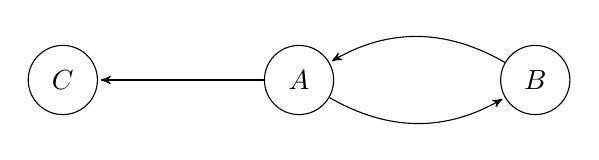
\begin{tikzpicture}[>=stealth',shorten >=1pt,node distance=3cm,on grid,initial/.style    ={}][!hb]
  \node[state]          (A)                        {$C$};
  \node[state]          (B) [right =of A]    {$A$};
  \node[state]          (C) [right =of B]    {$B$};

\tikzset{mystyle/.style={->}} 
\tikzset{every node/.style={fill=white}} 
\path (B)     edge [mystyle] (A)
      (B)     edge [bend right] [mystyle] (C) 
      (C)     edge [bend right] [mystyle] (B);
\end{tikzpicture}

DFS-with-timing on $G$ with the alphabetical order gives us the postlist $(A, C, B)$. If we redo DFS with the reverse of the postlist $(B, C, A)$ as a "magic ordering", it will start DFS with $B$ and the resulting $visited$ array is an array of all 1's. It means that $\{A, B, C\}$ is a connected component, which is not a true. \\


% Qimin
\q{10}{}
%\begin{enumerate}
%\item Given an undirected graph $G = (V, E)$, a vertex $t \in V$, and an edge $e = (u,v)\in E$, design a $O(|V|+|E|)$ time algorithm to determine whether there exists a cycle in $G$ that contains both $t$ and $e$.
Given a directed graph $G = (V, E)$, a vertex $t \in V$, and an edge $e = (u,v)\in E$, design
an $O(|V|+|E|)$ time algorithm to determine whether there exists a cycle in $G$ that contains both $t$ and $e$.
%\end{enumerate}

\textbf{Solution: }
We have that there exists a cycle in $G$ that contains both $t$ and $e$ if and only if
there exists a path from $v$ to $t$ and then from $t$ to $u$ in $G$. Therefore, we can design the following algorithm.

\emph{Algorithm.}
We run {\sf explore} twice.
The first run decides whether there exists a path from $v$ to $t$ in $G$. The
second run decides whether there exists a path from $t$ to $u$ in $G$. 
%We can initiate two BOOL {\sf b1} and {\sf b2} to store the result of the first run and the second run, respectively.  
For the first run, we run {\sf explore ($G$, $v$)}. If in the resulting {\sf visited} array we have {\sf visited[t] = 1}, (i.e., $t$ can be reached
from $v$ in $G$), then we continue the second run; otherwise the algorithm terminates and return that such cycle does not exist.
For the second run, we run {\sf explore ($G$, $t$)}. 
If in the resulting {\sf visited} array we have {\sf visited[u] = 1}, (i.e., $u$ can be reached from $t$ in $G$), then 
the algorithm returns that such cycle exists; otherwise 
there does not exist such a cycle.

\emph{Running Time.} 
Initiation of visited array runs $O(|V|)$ time. Run {\sf explore ($G$, $v$)} and {\sf explore ($G$, $t$)} both take $O(|E|)$ time. Therefore, the entire algorithm runs in $O(|V| + |E|)$ time.



% Tianyang
\q{10}{} Design an algorithm runs in $O(|V| + |E|)$ time which takes a directed graph as the input and determines if there is a vertex such that all other vertices are reachable from it.

\textbf{Solution: }\\
We can make the following observations before designing an algorithm:
\begin{itemize}
    \item \textbf{If such vertex exists, it must be in the connected component that is a source in the meta-graph} (which we'll call source connected component from now on). If it's in any non-source connected component, it wouldn't be able to reach to any vertex in a source connected component which contradicts with the requirement that all other vertices are reachable from that particular vertex.
    \item \textbf{There can only be one source connected component.} If there are multiple source connected components, a vertex in one source connected component wouldn't be able to reach a vertex in another source connected component which contradicts with the requirement as well.
\end{itemize}
With these observations, the algorithm simply needs to check if there is only one source connected component. There are multiple ways to do that:
\begin{itemize}
    \item Possible algorithm 1
    \begin{enumerate}
        \item Based on Claim 1 in lecture A11 typed note and the fact that any meta-graph is a DAG, we know that the vertex with the largest post number is in a source connected component after running DFS-with-timing. So, we do this and get that vertex i.e. the first vertex in the postlist. Time complexity: $\Theta(|V| + |E|)$. DFS-with-timing simply records pre, post numbers for each vertex and creates a postlist as it does DFS, so it still has the same running time as the regular DFS.
        \item Run \emph{explore} on that vertex. If all other vertices are visited in the procedure, the algorithm returns True. Otherwise, we know there is certain connected component that the source connected component containing that vertex can't reach. Since any meta-graph is a DAG, there must be at least one source connected component. Thus, it must be the case where there are multiple source components, and the algorithm can safely return False. Time complexity: $O(|V| + |E|)$.
    \end{enumerate}
    Overall, the running time is $O(|V| + |E|)$.
    \item Possible algorithm 2
    \begin{enumerate}
        \item Run the special version of DFS used to obtain all conncected components i.e. the algorithm mentioned in page 4 of lecture A11 typed note. Time complexity: $\Theta(|V| + |E|)$.
        \item Go through array \emph{visited} to find the vertices assigned with the largest $num{\text -}cc$. They consist of a source connected component. Time complexity: $\Theta(|V|)$.\\
        Correctness: The connected component containing these vertices is the last connected component we found. This implies that if we find all connected components by iteratively removing a sink connected component in the graph (as mentioned in page 3 of lecture A10 typed note), this particular connected component would be the last connected component remaining. Essentially, it is a source connected component since all non-source connected component would be removed before a source connected component.
        \item Same as step 2 in possible algorithm 1. Pick any vertex we found in the previous step and run \emph{explore} on that vertex.
    \end{enumerate}
    Overall, the running time is $O(|V| + |E|)$.
    \item Possible algorithm 3
    \begin{enumerate}
        \item Same as step 1 in possible algorithm 2.
        \item Construct the meta-graph for the given graph. More specifically, $V_m = \{C_1, \dots, C_n\}$, assuming $num{\text -}cc = n$ in the end. For all $(u, v) \in E$, add $(C_u, C_v)$ to $E_m$, assuming $C_u$ is the connected component containing $u$ and $C_v$ is the connected component containing $v$. Time complexity: $\Theta(|E|)$. Note that we don't need to go through array \emph{visited} or $V$.
        \item Go through $E_m$ to find the in-degree of all vertices in the meta-graph. The vertices with in-degree 0 represent source connected components. If there is only one vertex with in-degree 0, the algorithm returns True. Otherwise, it returns False. Time complexity: $O(|E|)$ since $|E_m| \le |E|$.
    \end{enumerate}
    Overall, the running time is $O(|V| + |E|)$.
\end{itemize}


% Manohar
\q{12}{} Run the strongly connected components algorithm on the following directed graphs G. When doing DFS on $G^R$: whenever there is a choice of vertices to explore, always pick the one that is alphabetically first.
\\\\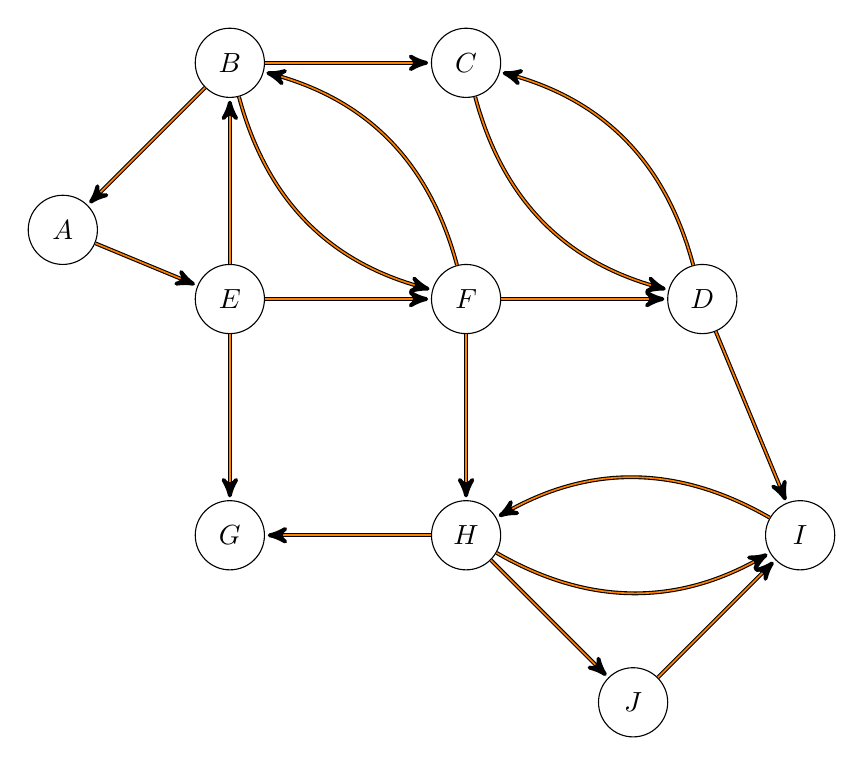
\begin{tikzpicture}[>=stealth',shorten >=1pt,node distance=3cm,on grid,initial/.style    ={}][!hb]
  \node[state]          (A)                        {$A$};
  \node[state]          (B) [above right =of A]    {$B$};
  \node[state]          (C) [right =of B]    {$C$};
  \node[state]          (F) [below =of C]    {$F$};
  \node[state]          (D) [right =of F]    {$D$};
  \node[state]          (E) [below =of B]    {$E$};
  \node[state]          (G) [below =of E]    {$G$};
  \node[state]          (H) [right =of G]    {$H$};
  \node[state]          (J) [below right =of H]   {$J$};
  \node[state]          (I) [above right =of J]    {$I$};
  

\tikzset{mystyle/.style={->,double=orange}} 
\tikzset{every node/.style={fill=white}} 
\path (B)     edge [mystyle] (A)
      (A)     edge [mystyle] (E) 
      (B)     edge [mystyle] (C)
      (B)     edge [bend right] [mystyle] (F)
      (F)     edge [bend right] [mystyle] (B)
      (C)     edge [bend right] [mystyle] (D)
      (D)     edge [bend right] [mystyle] (C)
      (D)     edge [mystyle] (I)
      (E)     edge [mystyle] (B)
      (E)     edge [mystyle] (F)
      (E)     edge [mystyle] (G)
      (F)     edge [mystyle] (D)
      (F)     edge [mystyle] (H)
      (H)     edge [mystyle] (G)
      (J)     edge [mystyle] (I)
      (H)     edge [mystyle] (J)
      (H)     edge [bend right] [mystyle] (I)
      (I)     edge [bend right] [mystyle] (H); 
\end{tikzpicture}
\begin{enumerate}
    \item Give the pre and post number of each vertex in the reverse graph $G^R$.
    \item In what order are the connected components found?
    \item Which are source connected components and which are sink connected components?
    \item Draw the ``metagraph'' (each meta-node is a connected component of $G$).
    \item What is the minimum number of edges you must add to $G$ to make it strongly connected?
\end{enumerate}

\textbf{Solution:} Reverse graph $G^R$ is as follows,

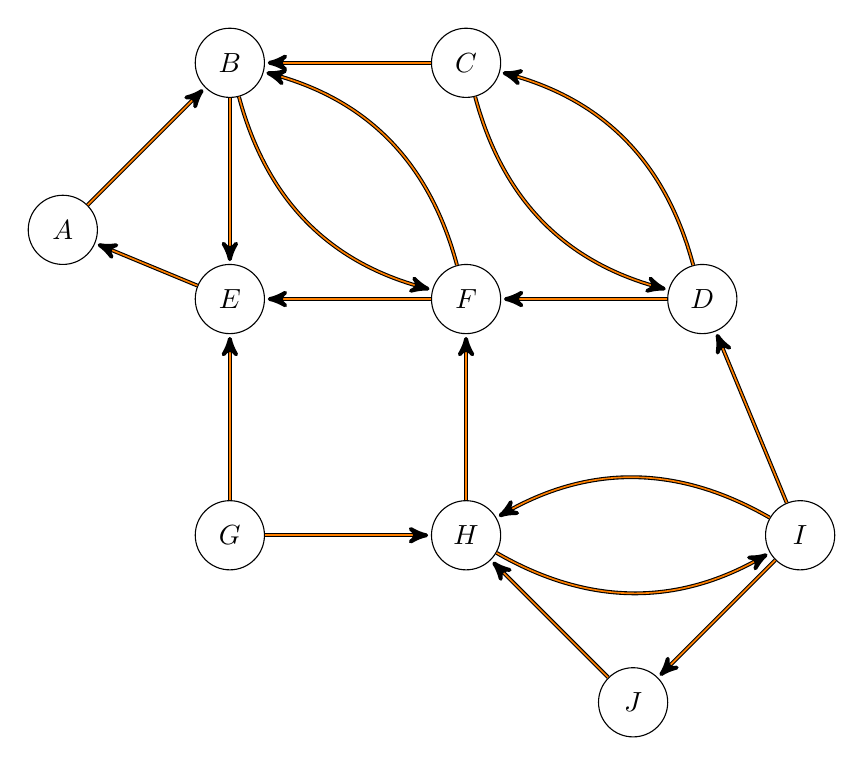
\begin{tikzpicture}[>=stealth',shorten >=1pt,node distance=3cm,on grid,initial/.style    ={}][!hb]
  \node[state]          (A)                        {$A$};
  \node[state]          (B) [above right =of A]    {$B$};
  \node[state]          (C) [right =of B]    {$C$};
  \node[state]          (F) [below =of C]    {$F$};
  \node[state]          (D) [right =of F]    {$D$};
  \node[state]          (E) [below =of B]    {$E$};
  \node[state]          (G) [below =of E]    {$G$};
  \node[state]          (H) [right =of G]    {$H$};
  \node[state]          (J) [below right =of H]   {$J$};
  \node[state]          (I) [above right =of J]    {$I$};
  

\tikzset{mystyle/.style={->,double=orange}} 
\tikzset{every node/.style={fill=white}} 
\path (A)     edge [mystyle] (B)
      (E)     edge [mystyle] (A) 
      (C)     edge [mystyle] (B)
      (F)     edge [bend right] [mystyle] (B)
      (B)     edge [bend right] [mystyle] (F)
      (C)     edge [bend right] [mystyle] (D)
      (D)     edge [bend right] [mystyle] (C)
      (I)     edge [mystyle] (D)
      (B)     edge [mystyle] (E)
      (F)     edge [mystyle] (E)
      (G)     edge [mystyle] (E)
      (D)     edge [mystyle] (F)
      (H)     edge [mystyle] (F)
      (G)     edge [mystyle] (H)
      (I)     edge [mystyle] (J)
      (J)     edge [mystyle] (H)
      (H)     edge [bend right] [mystyle] (I)
      (I)     edge [bend right] [mystyle] (H); 
\end{tikzpicture}
\begin{enumerate}
    \item pre and post numbers in $G^R$\\
    A : 1, 8\\
    B : 2, 7\\
    C : 9, 12\\
    D : 10, 11\\
    E : 3, 4 \\
    F : 5, 6 \\
    G : 13, 20\\
    H : 14, 19\\
    I : 15, 18\\
    J : 16, 17
    \item arranging the vertices in the decreasing order of post numbers,\\
    G, H, I, J, C, D, A, B, F, E\\
    Performing DFS on the given graph with above order will give us the connected components as follows,\\
    \{G\}, \{H, I, J\}, \{C, D\}, \{A, B, E, F\}
    \item Source connected components: \{A, B, E, F\}\\
    Sink connected components: \{G\}
    \item Meta graph of the given graph is as follows,\\
    \\\\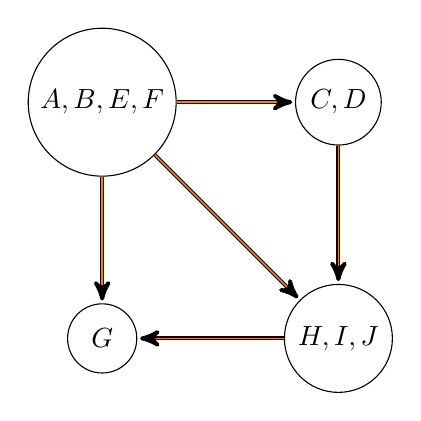
\begin{tikzpicture}[>=stealth',shorten >=1pt,node distance=3cm,on grid,initial/.style    ={}][!hb]
    \node[state]          (X)                        {$A, B, E, F$};
    \node[state]          (Y) [right =of X]    {$C, D$};
    \node[state]          (Z) [below =of X]    {$G$};
    \node[state]          (W) [below =of Y]    {$H, I, J$};
  

    \tikzset{mystyle/.style={->,double=orange}} 
    \tikzset{every node/.style={fill=white}} 
    \path (X)     edge [mystyle] (Y)
      (X)     edge [mystyle] (Z) 
      (W)     edge [mystyle] (Z)
      (Y)     edge [mystyle] (W)
      (X)     edge [mystyle] (W);
      \end{tikzpicture}
	  \item A graph is (strongly) connected means the meta-graph consists of a single vertex.
	  Therefore, we should add edges from all sink components to all source components.
	  Specifically, we can pick one vertex $u$ in a sink component and pick one vertex $v$ in a source component
	  and add an edge $(u,v)$, and we should do this for every pair of sink component and source component.
	  In this scenario there is only one sink component and one source component, So making an edge from
	  $G$ to one of the four vertices in $\{A, B, C, D\}$ will make the resulting graph connected.

\end{enumerate}
    
\newpage
{\huge {\bf Rubrics:}}

\bigskip


{\bf Problem 1, 10pts}
\begin{itemize}
    \item 5 points : Provided an appropriate counterexample, especially, the graph should be directed.
    \item 5 points : Provided an explanation with the postlist after the first DFS and the resulting $visited$ array.
    \item 1 point : I don’t know how to answer this question.
\end{itemize}

{\bf Problem 2, 10pts}
\begin{itemize}
    \item 10 points : correct algorithm
    \begin{itemize} 
    \item 3 points : appropriate explanation about twice explore
    \item 5 points : apply explore algorithm/DFS
    \item 2 points : correct return statements (e.g. return true if both b1 and b2 are true; otherwise return false) and running time analysis.
    \end{itemize}
    \item 1 point : I don't know how to answer this question
\end{itemize}

{\bf Problem 3, 10pts}
\begin{itemize}
    \item 2 points: Found out such vertex must be in a source connected component if it exists.
    \item 2 points: Found out the question is asking to find whether or not there is only one source connected component.
    \item 3 points: Provided a correct algorithm.
    \item 1 point: The provided algorithm has running time $O(|V| + |E|)$.
    \item 2 points: Provided a correct running time analysis.
    \item 1 point : I don’t know how to answer this question.
\end{itemize}

{\bf Problem 4, 12pts}
\begin{itemize}
    \item 3 points : correct pre and post numbers of the reverse graph 
    \item 3 points : correct connected components and their order.
    \item 1 point : correct source connected component (\{A, B, E, F\}).
    \item 1 point : correct sink connected component (\{G\}).
    \item 2 points : correct metagraph with 4 nodes and 5 edges.
    \item 1 point : one or more edges missing in the metagraph
    \item 2 point : identified that one edge need to be added (from sink to source).
    \item 1.2 point : I don't know how to answer this question.
\end{itemize}

\end{qunlist}
\end{document}
